% Preamble
\documentclass[a4paper, 12pt]{article}
\usepackage[margin=1in]{geometry} % Set margin
\usepackage{pdfpages} % Insert pdf pages
\usepackage{amssymb,amsmath,amsthm, amsfonts} % Math libraries

% Custom commands
\newcommand{\sub}[1]{\subsection{\underline{#1}}}
\newcommand{\subsub}[1]{\subsubsection{\underline{#1}}}
\newcommand{\R}{\ensuremath{\mathbb{R}}}
\newcommand{\F}{\ensuremath{\mathbb{F}}}
\newcommand{\N}{\ensuremath{\mathbb{N}}}
\newcommand{\Onef}{\ensuremath{1_{\F}}}
\newcommand{\Zerof}{\ensuremath{0_{\F}}}
\newcommand{\eqbcuz}[1]{\text{~$\stackrel{(#1)}{=}$~}}
\newcommand{\eq}[1]{\begin{align*}#1\end{align*}}
\newcommand{\eqn}[1]{\begin{align}#1\end{align}}
\newcommand{\set}[1]{\big{\{} #1 \big{\}}}
\newcommand{\bigset}[1]{\bigg{\{} #1 \bigg{\}}}
\renewcommand{\qed}{\hfill\(\qedsymbol\)}
\newtheorem{lemma}{Lemma}

% Begin Document %
\begin{document}

% Title Page
\begin{titlepage}
    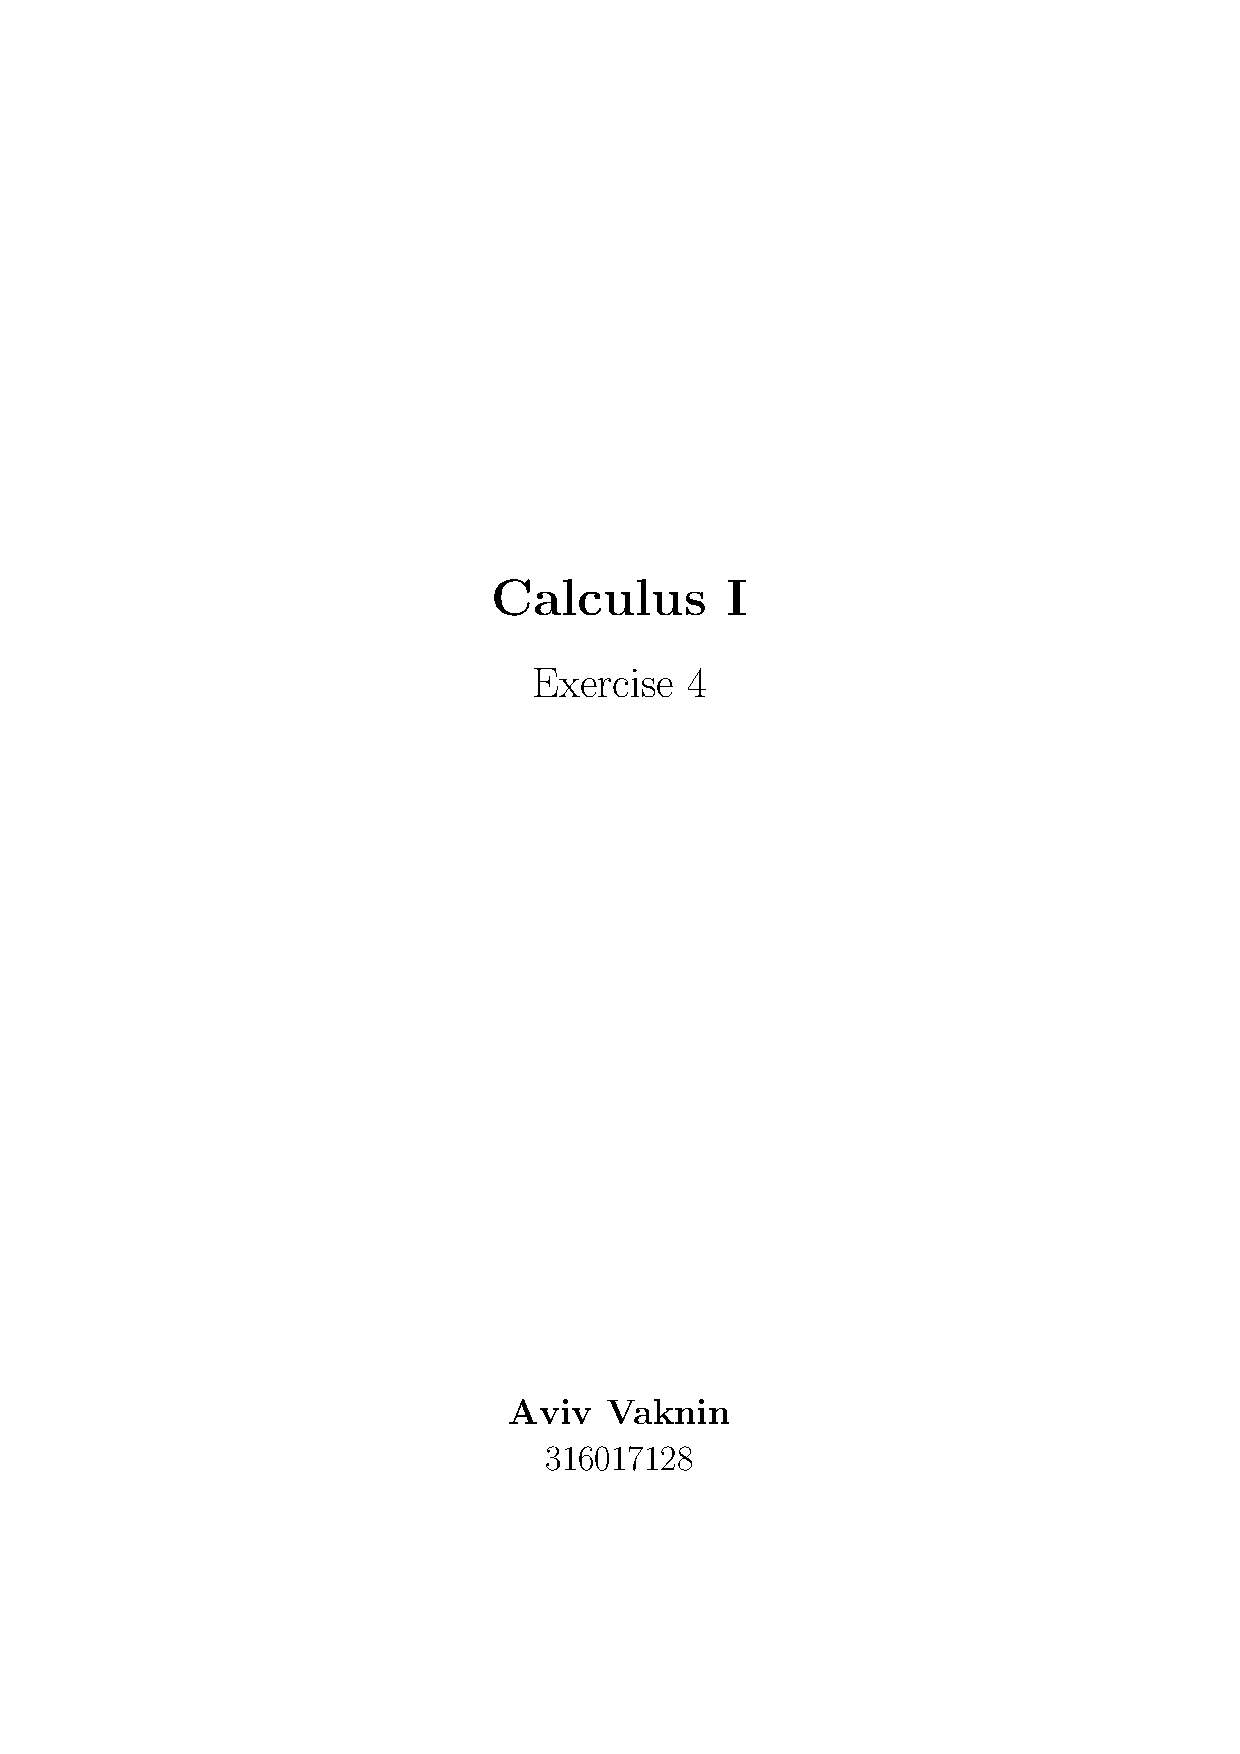
\includepdf{title.pdf}
\end{titlepage}

%1
\section{Prove \eq{
    \sup(\set{|x-y|~\big{|}~x,y\in{A}})=\sup{A}-\inf{A}
}}
First, let: \eq{D=\set{|x-y|~\big{|}~x,y\in{A}}}
We can see that \textit{D} consists of all of the distances in \textit{A}.\\
As we're searching for the supremum of this set, we're looking for the greatest \textit{x} and smallest \textit{y} values, that is:
\eq{
    x\in{A},~~x&=\max(A)\\
    y\in{A},~~y&=\min(A)\\
    |x-y|&=\max(D)
}
Possible candidates for min and max of a set, are the \textit{sup} and \textit{inf} of a set.\\
It is given that $A\in\R$, $A\neq\varnothing$ and that \textit{A} is bounded.\\
Therefore, according to the suprema and infima theorems, we can conclude that \textit{A} has a supremum and an infimum, such that:
\eq{
    &\sup(A)=s\\
    &\inf(A)=i
}
The only issue right now, is that \textit{s} and \textit{i} are unnecessarily part of \textit{A}.\\
Therefore, if we deduct or add some arbitrary $\frac{\epsilon}{2}>0$ from them, because of the definition of the supremum and infimum, they must be part of \textit{A}.
\eq{
    &x=\max(A)=s-\frac{\epsilon}{2}\\
    &y=\min(A)=i+\frac{\epsilon}{2}\\
    &x,y\in{A}
}
And therefore:
\eq{
    |x-y|=|s-\frac{\epsilon}{2}-(i+\frac{\epsilon}{2})|=|s-i-\epsilon|
}
According to definition, the supremum of a non-empty set must be greater than its infimum, therefore:
\eq{
    s&>i\\
    s&>i+\epsilon\\
    s-i-\epsilon&>0\\
    |s-i-\epsilon|&=s-i-\epsilon
}
Computing the supremum of D, we'll receive:
\eq{
    &\sup(D)=\sup(\{s-i-\epsilon\})=(s-i-\epsilon)+\epsilon=s-i\\
    &\sup(D)=\sup(A)-\inf(A)=s-i
}
\qed

%2
\section{Are the following subsets bounded from above or below? if yes, calculate the infimum/supremum, and decide whether there exist a min/max and compute them.}
\sub{}
\eq{
    A=\bigg{\{}
        \frac{3n+2}{n+5}~\bigg{|}~n\in\N
    \bigg{\}}
}
In order to work with this set, it'll be easier to first factor the term:
\eq{
    \frac{3n+2}{n+5}=\frac{3n+15}{n+5}-\frac{13}{n+5}=3-\frac{13}{n+5}
}
\subsub{lower-bound, infimum and minimum}
Now, it is easier to see that the term is smallest when $n=1$:
\eq{
    3-\frac{13}{6}=\frac{5}{6}
}
Thus, we can conclude that $i=\frac{5}{6}$ is the lower-bound, infimum and minimum of \textit{A}.
That is because $i\in{A}$, no other member of A is smaller than \textit{i}, and because it is the greatest lower-bound,
as if we'd increase its value, it would no longer be a lower-bound.
\subsub{higher-bound, supremum and maximum}
We can notice that as \textit{n} increases, the term $\frac{13}{n+5}$ is getting smaller and smaller, making the entire term closer and closer to 3.\\
Therefore, \textit{A} is bounded from above by 3, and it is its supremum as well.\\
However, \textit{A} does not have a maximum, because as n increases, the values get bigger.
\setcounter{subsection}{2}
\sub{}
\eq{
    C=\bigset{
        x\in\R~\big{|}~|x^2-4|\leq{5}
    }        
}
First, it is important to understand that $|x^2-4|\leq{5}$ implies that the only members that are in C fulfill:
\eq{
    \forall{c}\in{C}~-3\leq{c}\leq{3}
}
Therefore, it is quite easy to show that the lower-bound, infimum and minimum are -3,\\
while the higher-bound, supremum and maximum are 3.\\
That is because they exist in the set, no other member in the set is smaller or greater than them, and if we increase or decrease them, they will no longer be part of \textit{C}.
\qed\pagebreak

% 3
\section{Prove \eq{sup(A)=\sqrt{2}}}
In order to prove that $\sqrt{2}$ is the supremum of \textit{A}, we need to show:
    \begin{enumerate}
        \item \textit{A} is bounded from above by $\sqrt{2}$
        \item $\sqrt{2}$ is the smallest bound from above
    \end{enumerate}
% 3.1
\sub{$\sqrt{2}$ is the upper bound of \textit{A}}
The first part is almost immediate, as it is given that:
\eq{
    \forall{a}\in{A}~~a^2<2=\sqrt{2}^2
}
According to theorem 7.3 from class, we can say that:
\eq{
    a^2<\sqrt{2}^2\implies a<\sqrt{2}
}
Therefore, we can conclude that:
\eq{
    \forall{a}\in{A}~~a<\sqrt{2}
}
Thus, we've shown that $\sqrt{2}$ is the upper bound of \textit{A}.
% 3.2
\sub{$\sqrt{2}$ is the least-upper-bound of \textit{A}}
In order to show that $\sqrt{2}$ is the least-upper-bound of \textit{A},
we need to show that if we deduct \textit{any} arbitrary $\epsilon>0$ from it, the result will necessarily be a member of \textit{A}.\\
Let's suppose that there's a smaller upper-bound \textit{M} such that for some $0<\epsilon\in{Q}$:
\eq{
    M=\sqrt{2}-\epsilon<\sqrt{2}
}
Such an $\epsilon$ exists because we've proven that the rationals are dense in \R.\\
If we show that there exists an $a\in{A}$ such that $\sqrt{2}-\epsilon<a$, we'll show by definition that \textit{M} is not an upper-bound.
\eq{
    \sqrt{2},\sqrt{2}-\epsilon&>0\\
    \sqrt{2}-\epsilon&<\sqrt{2}
}
Because both sides of the inequality are greater than \textit{0}, we can square both of them:
\eq{
    (\sqrt{2}-\epsilon)^2&<(\sqrt{2})^2\\
    (\sqrt{2}-\epsilon)^2&<2
}
Every member \textit{q} of \textit{A} fulfills:
\eq{
q\in{Q} ~|~ (q>0) \land (q^2<2)
}
Therefore we've shown that $\sqrt{2}-\epsilon\in{A}$, and therefore \textbf{any} value that is lower than $\sqrt{2}$
cannot be the least-upper-bound of \textit{A}.
\qed\pagebreak

% 4
\section{}
% 4.1
\sub{$a,b\neq{0}~\land~n\in{Z} \implies (ab)^n=a^nb^n$}
We'll prove this using induction.\\
Because the induction is on $Z$ rather than $\N$, we'll check $n=0$ and $n=k-1$ as well.
\subsub{$n=0$:}
\eq{
    (ab)^0=1=1\cdot1=a^0b^0
}
\subsub{$n=k$:}
The induction assumption will be that it is true for any \textit{k}, that is:
\eq{
    (ab)^k=a^kb^k
}
\subsub{$n=k+1$:}
We'll start with power rules:
\eq{
    (ab)^{k+1}=(ab)^kab
}
And now we'll use our assumption:
\eq{
    (ab)^kab&=a^kb^kab\\
    &=a^kab^kb\\
    &=a^{k+1}b^{k+1}
}
\subsub{$n=k-1$:}
Power rules in $Z$:
\eq{
    (ab)^{k-1}=(ab)^k(ab)^{-1}
}
According to our induction assumption and some basic power rules that we've proved at (4.1):
\eq{
    (ab)^k(ab)^{-1}&=a^kb^k(ab)^{-1}\\
    &=\frac{a^kb^k}{ab}\\
    &=a^{k-1}b^{k-1}
}
\qed
% 4.2
\sub{$a,b>0~\land~r\in{Q} \implies (ab)^r=a^rb^r$}
\eq{
    r=\frac{k}{n} && k\in{Z} && n\in\N
}
We'll try to take the term $(ab)^r$ and mold it into another form:
\eq{
    ((ab)^r)^n&=\\
    &=((ab)^{\frac{k}{n}})^n\\
    &=(ab)^k\\
    &=a^kb^k
}
Notice that the last step was true because $k\in{Z}$.\\
Now, we'll do the same thing for $(a^rb^r)^n$:
\eq{
    (a^rb^r)^n&=\\
    &=(a^{\frac{k}{n}}b^{\frac{k}{n}})^n\\
    &=((a^k)^\frac{1}{n}(b^k)^\frac{1}{n})^n\\
}
Since $n\in\N\subset{Z}$, we can use the fact that we've just proved at (4.1).\\
\eq{
    ((a^k)^\frac{1}{n}(b^k)^\frac{1}{n})^n&=\\
    &=((a^k)^\frac{1}{n})^n((b^k)^\frac{1}{n})^n\\
    &=a^kb^k
}
Thus, we've shown:
\eq{
    ((ab)^r)^n=a^kb^k=(a^rb^r)^n
}
And therefore:
\eq{
    (ab)^r=a^rb^r
}
\qed

\pagebreak
% 6
\setcounter{section}{5}
\section{}
\pagebreak

% 7
\section{}
% 7.1
\sub{}
\eq{
    x_1,x_2&\in\R\\
    x_1, x_2&>0\\
    x_1x_2&=1
}
Prove:
    \eq{x_1+x_2\geq{2}}
We'll suppose by contradiction that:
\eq{
    x_1+x_2<2
}
Therefore:
\eq{
    x_1+x_2-2&<0\\
    x_1+\frac{1}{x_1}-2&<0
}
We'll multiply both sides of the inequality by $x_1$:
\eq{
    {x_1}^2-2x_1+1&<0\\
    (x_1-1)^2<0
}
Any element that is squared, cannot be less than 0.\\
Thus, we've reached a contradiction, which implies that our assumption was incorrect.
\qed

% 7.2
\sub{}
\subsub{Prove $1\leq{x_3}$ and $0<x_1\leq{1}$}
Let's assume both statements are false and show that a contradiction is given.\\
That is:
\eq{
    1-x_1&<0 & x_3-1&<0\\
    1&<x_1 & x_3&<1
}
Therefore, due to transitivity:
\eq{
    x_3<1<x_1
}
This is a contradiction to $x_1\leq{x_3}$, hence both statements are true.\\
Now, we'll show:
\eq{
    1+x_1x_3\leq{x_1+x_3}
}
We'll start with:
\eq{
    {1}&\leq{x_3}\\
    x_1x_2x_3&\leq{x_3}\\
}
We'll use the fact that $x_2=\frac{1}{x_1x_3}$ (because $x_1x_2x_3=1$) and we'll divide the above by $x_2$:
\eq{
    \frac{x_1x_2x_3}{x_2}\leq{x_3}\cdot{x_1x_3}
}
Therefore, we'll get:
\eqn{x_1x_3&\leq{x_1x_3x_3}}
If we add 1 (or its equivalent - $x_1x_2x_3$) to both sides of (1), we'll get:
\eqn{
    1+x_1x_3\leq{x_1x_2x_3}+x_1x_3x_3
}


Later:
\subsub{Prove $x_1+x_2+x_3\geq{3}$}


% End
\end{document}